\documentclass[a4paper, 12pt]{report}

%%%%%%%%%%%%
% Packages %
%%%%%%%%%%%%

\usepackage[english]{babel}
\usepackage[noheader]{packages/sleek}
\usepackage{packages/sleek-title}
\usepackage{packages/sleek-theorems}
\usepackage{packages/sleek-listings}
\usepackage{packages/seg-report-extra}
\usepackage{longtable}

\newcommand{\defaultInstructions}{
\begin{instructions}
Please remove all expectations and assessment environments from this page before submitting, including this instruction.  This is placeholder content to help you write the report.  It must not be included in the final report.
\end{instructions}
}

%%%%%%%%%%%%%%
% Title-page %
%%%%%%%%%%%%%%

\logo{./resources/pdf/Kcl-logo.pdf}
%\institute{Random University}
\faculty{Faculty of Natural, Mathematical, and Engineering Sciences}
\department{Department of Informatics}
\title{Software Engineering Group Project}
\subtitle{5CCS2SEG Major Group Project}%%% Insert project name here
\author{\textit{KCLMGP}\\   %%% Add team name here
Andrew Brown\\                        %%% Add first author here
Joshua Francis\\                        %%% Add second author here
Nour Hadhoud\\                      %%% Add three author here
Ziming Liu\\                       %%% Add four author here
Doris Nezaj\\           
Fasih-Ur Rahman\\                  %%% Add five author here
Hugo Potier de la Morandiere\\          %%% Add six
Scarlett Smith\\                      %%% Add seven author here
Ivan Tachev\\                      %%% Add eight author here
}
\date{\today}

%%%%%%%%%%%%%%%%
% Bibliography %
%%%%%%%%%%%%%%%%

\addbibresource{./resources/bib/references.bib}

%%%%%%%%%%
% Others %
%%%%%%%%%%

\lstdefinestyle{latex}{
    language=TeX,
    style=default,
    %%%%%
    commentstyle=\ForestGreen,
    keywordstyle=\TrueBlue,
    stringstyle=\VeronicaPurple,
    emphstyle=\TrueBlue,
    %%%%%
    emph={LaTeX, usepackage, textit, textbf, textsc}
}

\FrameTBStyle{latex}

\def\tbs{\textbackslash}

%%%%%%%%%%%%
% Document %
%%%%%%%%%%%%

\begin{document}
    \maketitle
    \romantableofcontents

    \chapter{Introduction}
\label{chap:introduction}
Our project aims to develop a dynamic and interactive habit tracking application that allows users to set and monitor personal and professional goals efficiently. By leveraging automation and data insights, the app will provide a seamless experience that minimises manual input, making habit tracking smarter and more intuitive. Users will also be able to gain valuable insights into their progress through clear visualisations, helping them stay motivated and accountable.

The application is designed as a cross-platform system, primarily for iOS users while also being accessible via the web. The app has been developed using React Native with Expo Go, utilising TypeScript and JavaScript, and backend by a MySQL database. By combining user activity tracking, geo-information, and screen monitoring, the app is able to intelligently record activities.

\defaultInstructions

\begin{expectations}
A good introduction gives the reader a good idea of what the project is about in the shortest amount of text.  A reader should be able to get through this chapter very quickly and decide whether this project is relevant to their interests.
\begin{itemize}
\item A summary of the overriding business objective of the application.  Explain what the client, the end-users of your application, or the organisation deploying it would gain from the application.  Explain this value from the perspective of the client's or users' world, not from your perspective as a developer.   Do not list features, requirements, or specifications here.  The software is a means to an end, not the objective in itself.
\item A statement of the type of system you built, including the platforms on which it can be used, and the technology stack used to build it.
\end{itemize}
This chapter does not require any sections of subsections.  In many projects, two short paragraphs will be enough.  However, you can use more if the objective cannot be explained in a single paragraph.  Note, though, that you will be developing the objectives further in the next chapter.
\end{expectations}

\begin{length}
A single page should be sufficient for this chapter.  More than two pages is too long.
\end{length}

    \chapter{Objectives and stakeholders}
\label{sect:objectives}

\defaultInstructions

\begin{length}
There are no strict length requirements for this chapter.  However, it is important that the writing is clear and concise.  Avoid repeating yourself.  It is expected that a typical project needs 1--3 pages, but this can vary considerably from project to project.
\end{length}

\begin{expectations}
This is a short chapter that identifies the objectives and stakeholders of the project.  A good report also discusses how the different types of stakeholder are affected by the project or how they could be affected by the project.

As you explain the project objectives, focus exclusively on what value the system adds to the stakeholders.  Your objectives should justify \emph{why} you are building the system.  The software requirements are \emph{not} objectives.  The software requirements explain \emph{what} your system can do.  In other words, they are a way to achieve objectives.  Software requirements do \emph{not} belong in this chapter.  Your project should have at least one objective.  Otherwise, the project is a pointless exercise.  Many objectives do not necessarily make for a better project.

Some stakeholders of a project will be obvious: e.g. the people who the beneficiaries of the value your project adds.  However, it is important to be aware of all stakeholders.  The stakeholder D.A.N.C.E. tool to identify all stakeholders and it is explained in a video on project initiation.  Consider carefully how each stakeholder is affected by your project and who the key stakeholders are.

The section headers below provide a suggested structure.  You should feel free to change it or extend it.
\end{expectations}

\section{Project objectives}
\label{sect:objectives}

\section{Stakeholder}
\label{sect:stakeholder}

\subsection{Stakeholder analysis}
\subsection{Key stakeholders}
    \chapter{Specifications}
\label{chap:specifications}

\defaultInstructions

\begin{length}
There are no strict length requirements for this chapter.  However, it is important that the writing is clear and concise.  Avoid repeating yourself.  It is expected that a typical project needs 1--5 pages, but this can vary considerably from project to project.
\end{length}

\begin{expectations}
This chapter should provide the specifications of the software that you have implemented.  Good specifications are clear, concise, consistent (with one another and with the project objectives), estimable (the effort required of functional requirements should be estimable), and testable (you should be able to create automated or manual tests for these specifications).

A significant part of this chapter covers functional requirements/specifications.  These refer to the product features your team has developed.  Present a clear overview of all functional requirements/specifications that can be found in the deployed system.  For each feature, explain how it contributes to the project objectives, and explain how/where it can be found.  Do \emph{not} mix the specifications the team managed to implement with those they did not.  

If necessary or helpful for clarity, explain what is out of scope of the project in a distinct section.  You may discuss ideas for functional specifications the team did not manage to implement, provided this discussion is clearly distinct from the project's achieved functional specifications.

The project objectives will also entail certain non-functional specifications.  These may include, for example, reliability, usability, portability, scalability, performance, compatibility, security, compliance, etc.  Identify which non-functional specifications are important to this project and define them.  Make sure to present them in order of importance, and relate each one to the project objectives.  

The section headers below provide a suggested structure.  You should feel free to change it or extend it.
\end{expectations}

\section{Functional specifications}
\label{sect:functional-specifications}
The following features have been developed and are accessible in the deployed application. Each contributes directly to the project's objectives of creating a flexible, user-friendly application that can enhance the user's productivity.

\subsection{Habit Creation and Management}
\subsubsection{Creating New Habits:}
\begin{itemize}
    \item \textbf{Description:} Users can create new habits with customisable details including name, description, type (build or quit), colour, schedule options, and optional goals.
    \item \textbf{Contribution to Objectives:} This is the core functionality that allows users to define specific behaviours they want to track, making the app personalized and adaptable to diverse habit-building needs.
    \item \textbf{Location:} On the habits page, which is the fist page that is shown on login, there is an add habit button which which takes you to a form. This form is used for the user to customise that habit that they are creating.
\end{itemize}

\subsubsection{Habit Types (Build vs Quit):}
\begin{itemize}
    \item \textbf{Description:} The app distinguishes between habits to build (positive behaviours to adopt) and habits to quit (negative behaviours to eliminate).
    \item \textbf{Contribution to Objectives:} This differentiation supports different behaviour change strategies and accommodates customisation of habits for the user.
    \item \textbf{Location:} On the habit page the user will be able to tell the difference between a quitting habit and a building habit. When the user is creating a habit using the form at the top of the form they will choose between a build or quit habit.
\end{itemize}

\subsubsection{Habit Customisation:}
\begin{itemize}
    \item \textbf{Description:} Users can customise habits with colour-coding, descriptions, and personal tracking parameters.
    \item \textbf{Contribution to Objectives:} Customisation enhances user engagement by allowing personal expression and visual organization of different habits.
    \item \textbf{Location:} All customisation of the habits can be done when the user presses the add habit button, which opens the form for the user to create their habit.
\end{itemize}

\subsubsection{Editing Existing Habits:}
\begin{itemize}
    \item \textbf{Description:} Users can modify all aspects of their habits after creation, including schedules, goals, and appearance.
    \item \textbf{Contribution to Objectives:} Allows flexibility as users refine their habits and tracking needs over time, preventing abandonment when circumstances change.
    \item \textbf{Location:} In the top right corner of every habit there is a little pencil icon. When it is pressed a form is open with pre-filled in data which the user can change to edit the habit to their liking.
\end{itemize}

\subsection{Scheduling and Frequency}
\subsubsection{Interval-Based Scheduling:}
\begin{itemize}
    \item \textbf{Description:} Users can set habits to repeat at regular intervals (every X days).
    \item \textbf{Contribution to Objectives:} Supports habits that don't follow a weekly pattern and accommodates varying frequency needs.
    \item \textbf{Location:} In the add habit and edit habit forms the user can choose to schedule the habit at regular intervals. So they enter a number for the habit to show every X days.
\end{itemize}

\subsubsection{Weekly Day-Based Scheduling}
\begin{itemize}
    \item \textbf{Description:} Users can schedule habits for specific days of the week (e.g., Monday, Wednesday, Friday).
    \item \textbf{Contribution to Objectives:} Accommodates routines that follow weekly patterns, supporting integration with typical work/life schedules.
    \item \textbf{Location:} In the add habit and edit habit forms the user can choose to schedule the habit by selecting days of the week. The user will highlight the days of the week they want the habit to appear.
\end{itemize}

\subsubsection{Instance Generation}
\begin{itemize}
    \item \textbf{Description:} The system automatically generates future instances of habits based on their scheduling patterns.
    \item \textbf{Contribution to Objectives:} Ensures users always have upcoming habits ready to track without manual creation.
    \item \textbf{Location:} Using the calendar at the top of the habits page, the user can select future days of the week to see the habit they will have to complete. The user can also check the habits on dates that are on future weeks.
\end{itemize}

\subsection{Goal Setting and Tracking}
\subsubsection{Numeric Goal Setting}
\begin{itemize}
    \item \textbf{Description:} For "build" habits, users can set specific numeric goals with custom units (e.g., read 30 pages, meditate 20 minutes).
    \item \textbf{Contribution to Objectives:} Provides clear, measurable targets that make progress tracking more concrete and satisfying.
    \item \textbf{Location:} Clicking on the habit will allow the user to enter how much progress they have made so far on the habit.
\end{itemize}

\subsubsection{Binary Completion Tracking}
\begin{itemize}
    \item \textbf{Description:} For "quit" habits, users track success with yes/no completion options.
    \item \textbf{Contribution to Objectives:} Simplifies tracking for avoidance-based habits where the goal is simply not engaging in a behaviour.
    \item \textbf{Location:} Clicking on the habit will allow the user to enter if they have completed the habit or not.
\end{itemize}

\subsubsection{Progress Recording}
\begin{itemize}
    \item \textbf{Description:} Users can record daily progress toward habit goals including partial completion.
    \item \textbf{Contribution to Objectives:} Encourages consistent habit engagement by acknowledging incremental progress rather than all-or-nothing success.
    \item \textbf{Location:} Clicking on the habit will allow the user to enter how much progress they have made so far on the habit.
\end{itemize}

\subsubsection{Habit Streak Tracking}
\begin{itemize}
    \item \textbf{Description:} Each habit has a streak of how many days in a row the user has fully completed the habit.
    \item \textbf{Contribution to Objectives:} This encourages the user to keep up with their habits as the larger their streak goes, the harder the user will try to keep it going.
    \item \textbf{Location:} The streak is shown by a fire icon, followed by a number (the number of days the streak is on). It's found on every habit next to the edit habit button.
\end{itemize}

\subsection{Visualisation and Statistics}
\subsubsection{Calendar View}
\begin{itemize}
    \item \textbf{Description:} Provides a monthly calendar visualization showing total habit completion of each day for the month.
    \item \textbf{Contribution to Objectives:} Gives users a holistic view of their habit consistency, helping identify patterns and trends.
    \item \textbf{Location:} This can be found on the calendar page which can be accessed using the menu at the bottom of the screen.
\end{itemize}

\subsubsection{Average Completion Percentage}
\begin{itemize}
    \item \textbf{Description:} Shows the average completion percentage of each day for the whole month
    \item \textbf{Contribution to Objectives:} Provides a quick measure of overall habit success to allow the user to track their progress.
    \item \textbf{Location:} There is a circle at the bottom of the calendar on the calendar page that shows the average completion percentage for that month.
\end{itemize}

\subsubsection{Daily Streak Tracking}
\begin{itemize}
    \item \textbf{Description:} Records and displays the current and longest streak of consecutive days with all the habit fully completed.
    \item \textbf{Contribution to Objectives:} This encourages the user to keep up with their habits as the larger their streak goes, the harder the user will try to keep it going.
    \item \textbf{Location:} The streaks are found in between the monthly calendar and the average completion percentage circle, on the calendar page.
\end{itemize}

\subsection{Date Navigation and Filtering}
\subsubsection{Weekly Calendar Navigation}
\begin{itemize}
    \item \textbf{Description:} A scrollable weekly calendar view allowing selection of specific dates to view and manage habits
    \item \textbf{Contribution to Objectives:} Provides intuitive temporal navigation for managing habits on different days.
    \item \textbf{Location:} On the habits page at the top of the screen.
\end{itemize}

\subsubsection{Date-Specific Habit Filtering}
\begin{itemize}
    \item \textbf{Description:} Displays only relevant habits for the selected date based on scheduling rules.
    \item \textbf{Contribution to Objectives:} Reduces cognitive load by showing only what's relevant for the current day or selected date.
    \item \textbf{Location:} By using the weekly calendar on the habits page the habits that are displays will only be relevant to the date selected.
\end{itemize}

\subsection{Data Persistence and Synchronization}
\subsubsection{User Authentication}
\begin{itemize}
    \item \textbf{Description:} Secure user account system with email-based authentication.
    \item \textbf{Contribution to Objectives:} Protects user data and enables personalized habit tracking.
    \item \textbf{Location:} The user can create an account using the sign in page. If they already have an account they can use the login page to login to their account.
\end{itemize}

\subsection{User Interface Features}
\subsubsection{Theme Support}
\begin{itemize}
    \item \textbf{Description:} Application supports light and dark themes with appropriate colour schemes.
    \item \textbf{Contribution to Objectives:} Enhances user experience and accessibility in different lighting conditions and according to user preference.
    \item \textbf{Location:} The user can switch between light and dark mode using a selector that can be found in the settings page.
\end{itemize}

\subsubsection{Responsive Design}
\begin{itemize}
    \item \textbf{Description:} UI adapts to different screen sizes and orientations.
    \item \textbf{Contribution to Objectives:} Ensures a consistent experience across different devices.
    \item \textbf{Location:} This is found through out the whole app.
\end{itemize}

\section{Non-functional specifications}
\subsection{Security}
\subsubsection{Password Hashing}
\begin{itemize}
    \item \textbf{Description:} User passwords are securely hashed before storage.
    \item \textbf{Contribution to Objectives:} Protects user credentials even in case of a data breach.
    \item \textbf{Location:} All of the hashing is done on the client side so only the hashed password gets stored on the server side.
\end{itemize}

\subsection{Reliability}
\subsubsection{Error Handling}
\begin{itemize}
    \item \textbf{Description:} Comprehensive error handling for all API calls and user interactions.
    \item \textbf{Contribution to Objectives:} Ensures graceful failure and prevents app crashes when operations fail.
    \item \textbf{Location:} Can be found throughout the app.
\end{itemize}

\subsection{Usability}
\subsubsection{Intuitive UI Elements}
\begin{itemize}
    \item \textbf{Description:} User interface designed with intuitive controls and visual feedback.
    \item \textbf{Contribution to Objectives:} Reduces learning curve and improves user experience.
    \item \textbf{Location:} Can be found throughout the app.
\end{itemize}

\subsubsection{Form Validation}
\begin{itemize}
    \item \textbf{Description:} Input validation for all user-submitted data.
    \item \textbf{Contribution to Objectives:} Prevents errors from invalid data and provides immediate feedback.
    \item \textbf{Location:} Can be found throughout the app (e.g., logging in or signing in, creating or editing a habit, inputting habit progress, etc.)
\end{itemize}

\subsection{Maintainability}
\subsubsection{Modular Architecture}
\begin{itemize}
    \item \textbf{Description:} Code organized into reusable, single-responsibility components.
    \item \textbf{Contribution to Objectives:} Simplifies maintenance and enables easier feature additions or modifications.
    \item \textbf{Location:} Found throughout all the files in the code.
\end{itemize}

\subsubsection{Typescript Implementation}
\begin{itemize}
    \item \textbf{Description:} Strong typing throughout the application using Typescript.
    \item \textbf{Contribution to Objectives:} Catches type-related errors at compile time and improves code documentation.
    \item \textbf{Location:} Used throughout the code.
\end{itemize}

\subsection{Compatibility}
\subsubsection{Cross-platform Support}
\begin{itemize}
    \item \textbf{Description:} Implemented using React Native to work across different device types.
    \item \textbf{Contribution to Objectives:} Provides consistent user experience on iOS, Android, and potentially web platforms.
    \item \textbf{Location:} React Native components are used throughout the code.
\end{itemize}

\subsection{Data Management}
\subsubsection{Efficient Data Storage}
\begin{itemize}
    \item \textbf{Description:} Optimized database schema with appropriate relationships and indexing.
    \item \textbf{Contribution to Objectives:} Minimizes storage requirements while maintaining data integrity.
    \item \textbf{Location:} Found in the server.js file in the project code.
\end{itemize}

\subsubsection{Offline Capability}
\begin{itemize}
    \item \textbf{Description:} Progress data and account details for the use is saved even when the app is closed.
    \item \textbf{Contribution to Objectives:} Allows user to access account on different devices
    \item \textbf{Location:} Data is saved on a cloud database.
\end{itemize}

\label{sect:non-functional-specifications}

    \chapter{Project management}
\label{chap:project-management}

\defaultInstructions

\begin{length}
There are no strict length requirements for this chapter.  However, it is important that the writing is clear and concise.  Avoid repeating yourself.  Make sure to clearly signpost evidence for claims.  It should be possible for a reader to understand this chapter without consulting other sources.  It is expected that a typical project needs 3--6 pages, but this can vary considerably from project to project.
\end{length}

\begin{expectations}
In this chapter, the team must present, reflect on, and evaluate the team's approaches to project management.  This discussion should present the main approaches to project management the team decided to use.  Include the team's rationale for these decisions, and the team's observations on the effectiveness of each approach.

During the project, the team may have made significant changes to project management approaches, or made new decisions where initial arrangements were insufficient.  A typical team will also have encountered difficulties, such as risks that materialised and impacted the team.  Discuss the most critical decisions the team made, why you made them, and what the results were.  If certain approaches were not entirely successful, discuss what you would do differently in a future project.  

A good report shows a systematic approach to project management, justifications for key decisions, and a critical reflection on the effectiveness of different approaches.  Ideally, the justifications and reflections in this chapter are based on project management theory.

Note that ``a systematic approach to project management'', ``critical reflection'', and use of ``project management theory'' do not necessary imply that your team's project management approach is a success story.  Thoughful, considered project management improves your chances of success, but projects do not always go according to plan and team's make mistakes.  The markers are looking for 
\begin{itemize}
    \item Good justifications for approaching a project in a particular way.
    \item Critical reflection on the results, including recognition of problems.
    \item The team taking ownership of the problems they encountered.
\end{itemize}

There is no one best way of organising this content.  One approach is to cover different phases of the project management lifecycle (from initialisation to project close).  Another approach is to cover different project management tasks (e.g. team management, scheduling, planning, risk, etc.).  Yet another approach is to cover the most impactful events.  Each project is different and you should take the approach that works best for your team.

There is also no minimum or maximum number of issues to cover.  Cover what is more important in the depth necessary to do the topic justice.
\end{expectations}

\subsection{Project Overview and Scope}
During initiation, we formally agreed on the project scope as captured in our scope statement. The primary outcome of this phase was to gain clarity on what our application would and would not include. We found this step highly effective at allowing us to understand the true value we want to provide, which allowed us to implement features that are coherent and make sense. Identifying stakeholders early was also key to gain clarity on who we are providing value to. Below are some of the key decisions made during our first two project initiation meetings in week 1.

\subsubsection{Project Purpose and Description}
A mobile-web hybrid application that provides a flexible way for users to track their habits. The app will help users enforce new good habits and assist with ending bad habits. By offering clear data visualisations, a user-friendly interface, and customisable habits, the system helps users manage their goals.

\subsubsection{Desired Results and Exclusions}
\textbf{In Scope:}
\begin{itemize}
    \item Building a habit and activity tracking app using React Native with Expo Go, TypeScript/JavaScript, and a MySQL database.
    \item Allowing users to register/log in, set custom habit goals, and track progress.
    \item Providing clear data visualisations (charts, graphs, analytics) and a data export feature.
\end{itemize}

\textbf{Exclusions:}
\begin{itemize}
    \item Frequent reminders or push notifications are out of scope; notifications will be weekly.
    \item Direct integration with third-party apps/services.
\end{itemize}

\subsubsection{Constraints}
\textbf{Time:} The project must be completed within a 10-week window (13/01/25 – 27/03/25).\\
\textbf{Team Size:} There are 9 group members, requiring effective communication to manage coordination.\\
\textbf{Skill Sets:} The team’s familiarity with React Native, Expo Go, TypeScript, and MySQL may limit feature complexity.\\
\textbf{Workload Balance:} The team must juggle other academic responsibilities alongside this development project.

\subsection{Stakeholder Identification}
We used the D.A.N.C.E. framework to classify stakeholders, as detailed in Chapter 2 of this report. At this stage, we focused on:
\begin{itemize}
    \item \textbf{Primary Users} - those who directly interact with the app.
    \item \textbf{Development Team} - responsible for planning, designing, building, and deployment.
    \item \textbf{Academic Supervisors} - providing guidance and evaluation.
\end{itemize}

\subsection{Our Project Management Approach}
Initially, we agreed to combine Agile techniques (e.g., using Trello with story points) with a more traditional Waterfall Model (e.g., a fixed final deadline, staged deliverables). This hybrid approach provided us with:
\begin{itemize}
    \item Flexibility to reprioritise features when faced with new insights or changing team availability.
    \item Structure to ensure mandatory deliverables (e.g., report chapters, final submission) meet set deadlines.
\end{itemize}

\section{Planning}
Planning was critical in laying out how we would achieve the objectives defined in our scope statement. As recommended by project management theory (PMBOK, 2017), we focused on risk management, scheduling, and communication planning.

\subsection{Risk Management}
We identified potential risks early on and agreed on their probability and impact. Identifying risks early allowed us to understand how to quickly minimise problems when they would inevitably arise, helping us waste less time. For example, as seen in Table 4.1., one risk we identified was "Missed deadlines" which led us to understand the importance of setting weekly task deadlines in our project.

\begin{table}[H]
    \centering
    \caption{Project Risk Management (source: Team Feedback Meeting Minutes 29/01/25)}
    \label{table:project_risk}
    \begin{tabular}{|p{5cm}|c|c|p{6cm}|}
        \hline
        \textbf{Risk} & \textbf{Probability} & \textbf{Impact} & \textbf{Mitigation} \\
        \hline
        Poor team communication & Medium & High & Establish a weekly meeting date (Wednesdays) and communicate regularly using Discord. \\
        \hline
        Missed deadlines & Medium & High & Use Trello regularly, assign deadlines to each task, and keep the group updated. \\
        \hline
        Deployment and Hosting issues & Low & High & Choose a reliable hosting provider. Test deployment. \\
        \hline
        Delays caused by dependencies in code development & Medium & High & Assign tasks thoughtfully and keep the group updated with tasks. \\
        \hline
        Technical issues & Medium & High & Make sure to test regularly. Regular communication with the team. \\
        \hline
    \end{tabular}
\end{table}

We also re-evaluated risks during the project review meeting, which was effective at helping us identify where we were falling behind as a team, such as addressing security issues (see Figure \ref{fig:reeval_risks}). (See Section 4.3 for a further evaluation of our project review meeting).

\begin{figure}[H]
    \centering
    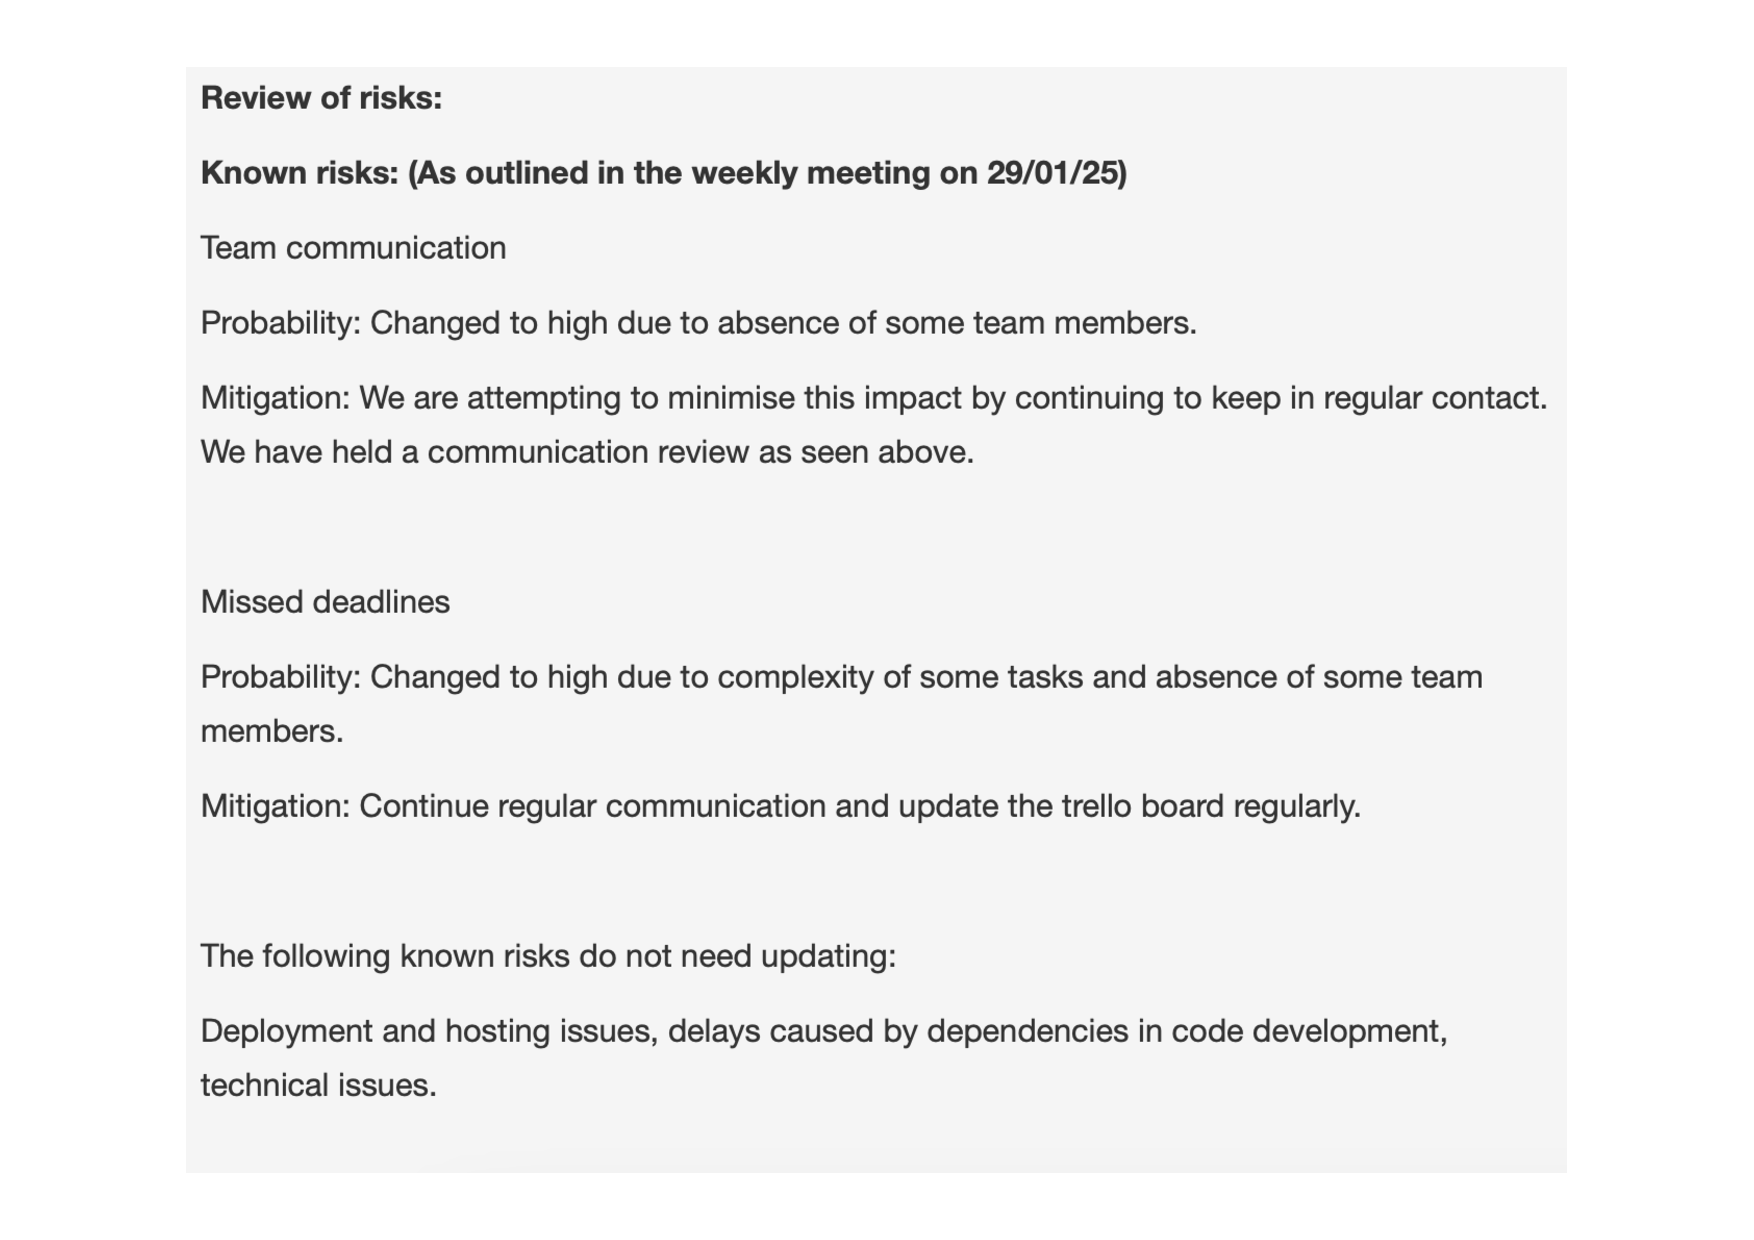
\includegraphics[width=0.9\textwidth]{resources/risk_review.pdf}
    \caption{Reevaluation of Risks (source: Team Feedback Meeting Minutes 26/02/25)}
    \label{fig:reeval_risks}
\end{figure}

\subsection{Scheduling}
Our scheduling used Trello to break down epics into manageable tasks. We assigned story points on a scale of 1 to 5. This allowed us to:
\begin{itemize}
    \item Estimate the project velocity (around 15 story points/week during our project review meeting).
    \item Track our backlog of tasks and ensure we were on track for submission by the deadline.
\end{itemize}

\begin{figure}[H]
    \centering
    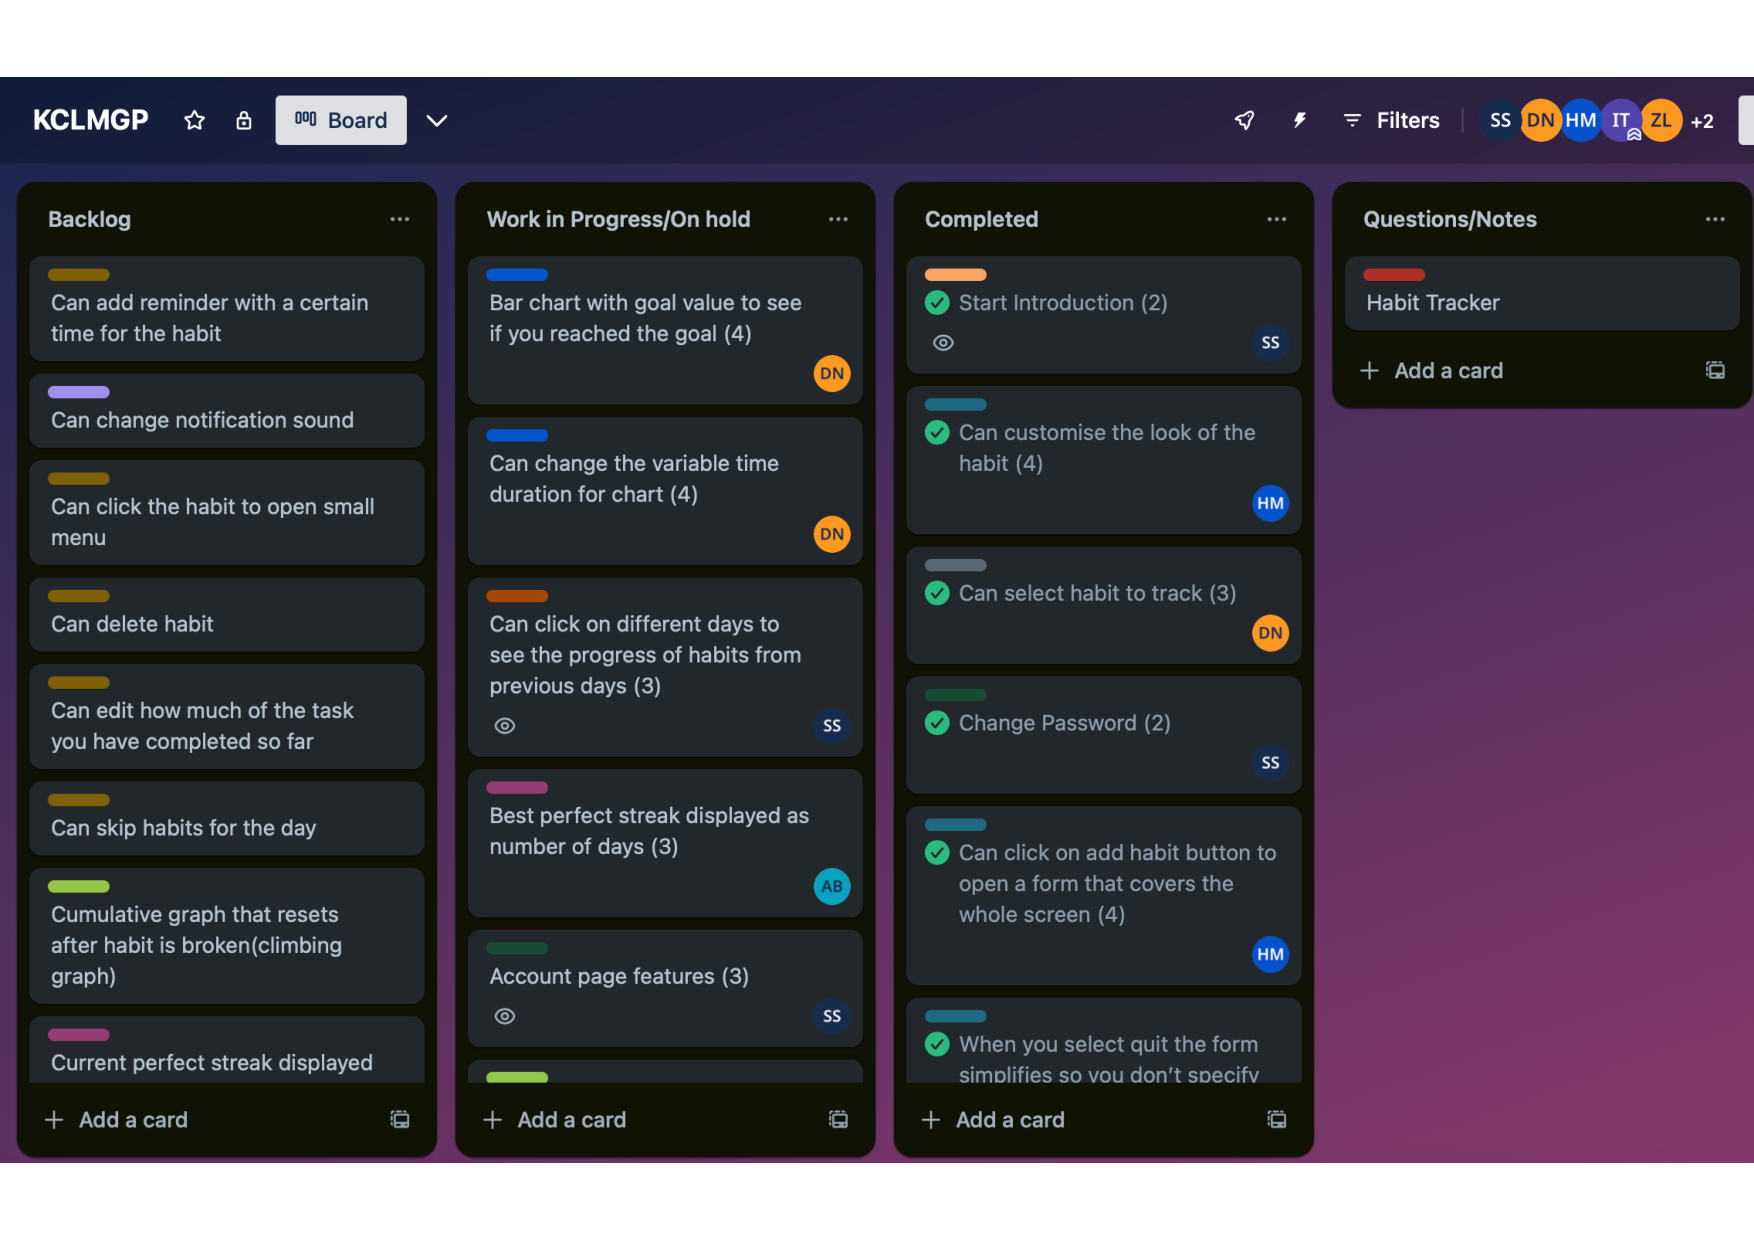
\includegraphics[width=0.8\textwidth]{resources/trello_board.pdf}
    \caption{Screenshot of Trello board showing tasks and progress}
    \label{fig:trello_tasks}
\end{figure}

As seen in Figure \ref{fig:trello_tasks}, something we would improve in the future is to include a ‘Testing’ section on our Trello board. This would have ensured that all tasks marked as ‘complete’ were thoroughly tested beforehand, preventing bugs and the need for retrospective testing.

One aspect that we agreed worked well was using colour-coded labels for each task (see Figure \ref{fig:trello_tasks}), which allowed us to separate different areas of our app. This helped organise task allocation and reduced dependencies in code development, which addressed one of our ‘High’ impact risks (see Table \ref{table:project_risk}).

\begin{figure}[H]
    \centering
    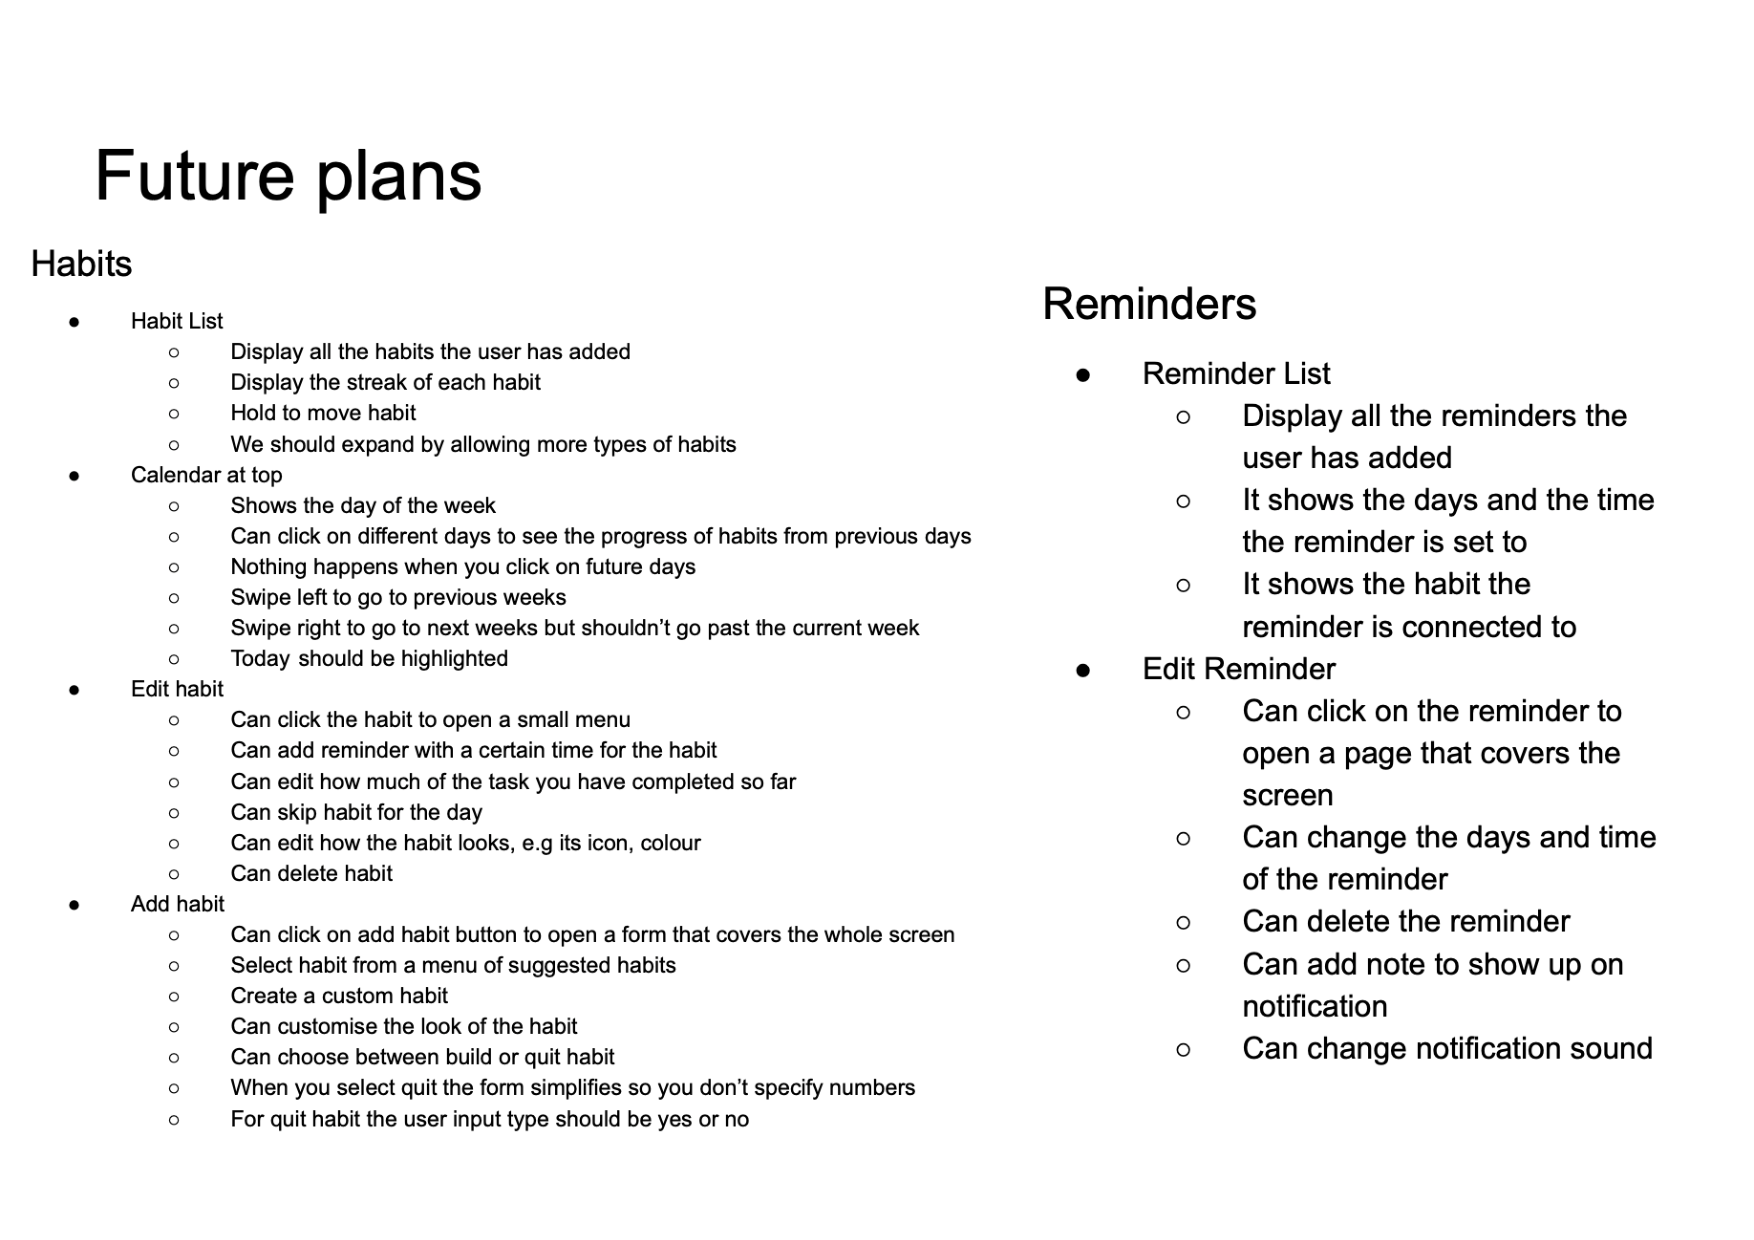
\includegraphics[width=0.8\textwidth]{resources/task_list.pdf}
    \caption{Page 1 of our backlog of organised tasks defined during the Week 2 Planning meeting (28/01/25)}
    \label{fig:task_list}
\end{figure}

\subsection{Communication Planning}
We formally agreed on the following communication strategies (as recorded in Team Feedback Meeting Minutes 29/01/25):

\begin{itemize}
    \item \textbf{Weekly Team Meetings:} Every Wednesday, in FWB Library.
    \begin{itemize}
        \item Discuss tasks completed, tasks in progress, and next steps.
    \end{itemize}
    \item \textbf{Online Communication (Discord):} For quick updates, online meetings, and working together on tasks.
    \item \textbf{Team Feedback \& GitHub Integration:} We used Team Feedback to share commits and attribute coding work. Collaborative coding sessions were recorded to ensure proper credit distribution.
\end{itemize}

One aspect of communication that we found effective and would implement again is the use of different communication channels on Discord. This allowed us to organise and manage our online discussions effectively, ensuring all saved materials were in one place and weekly targets were clearly communicated (see Figure \ref{fig:discord_channels}).

\begin{figure}[H]
    \centering
    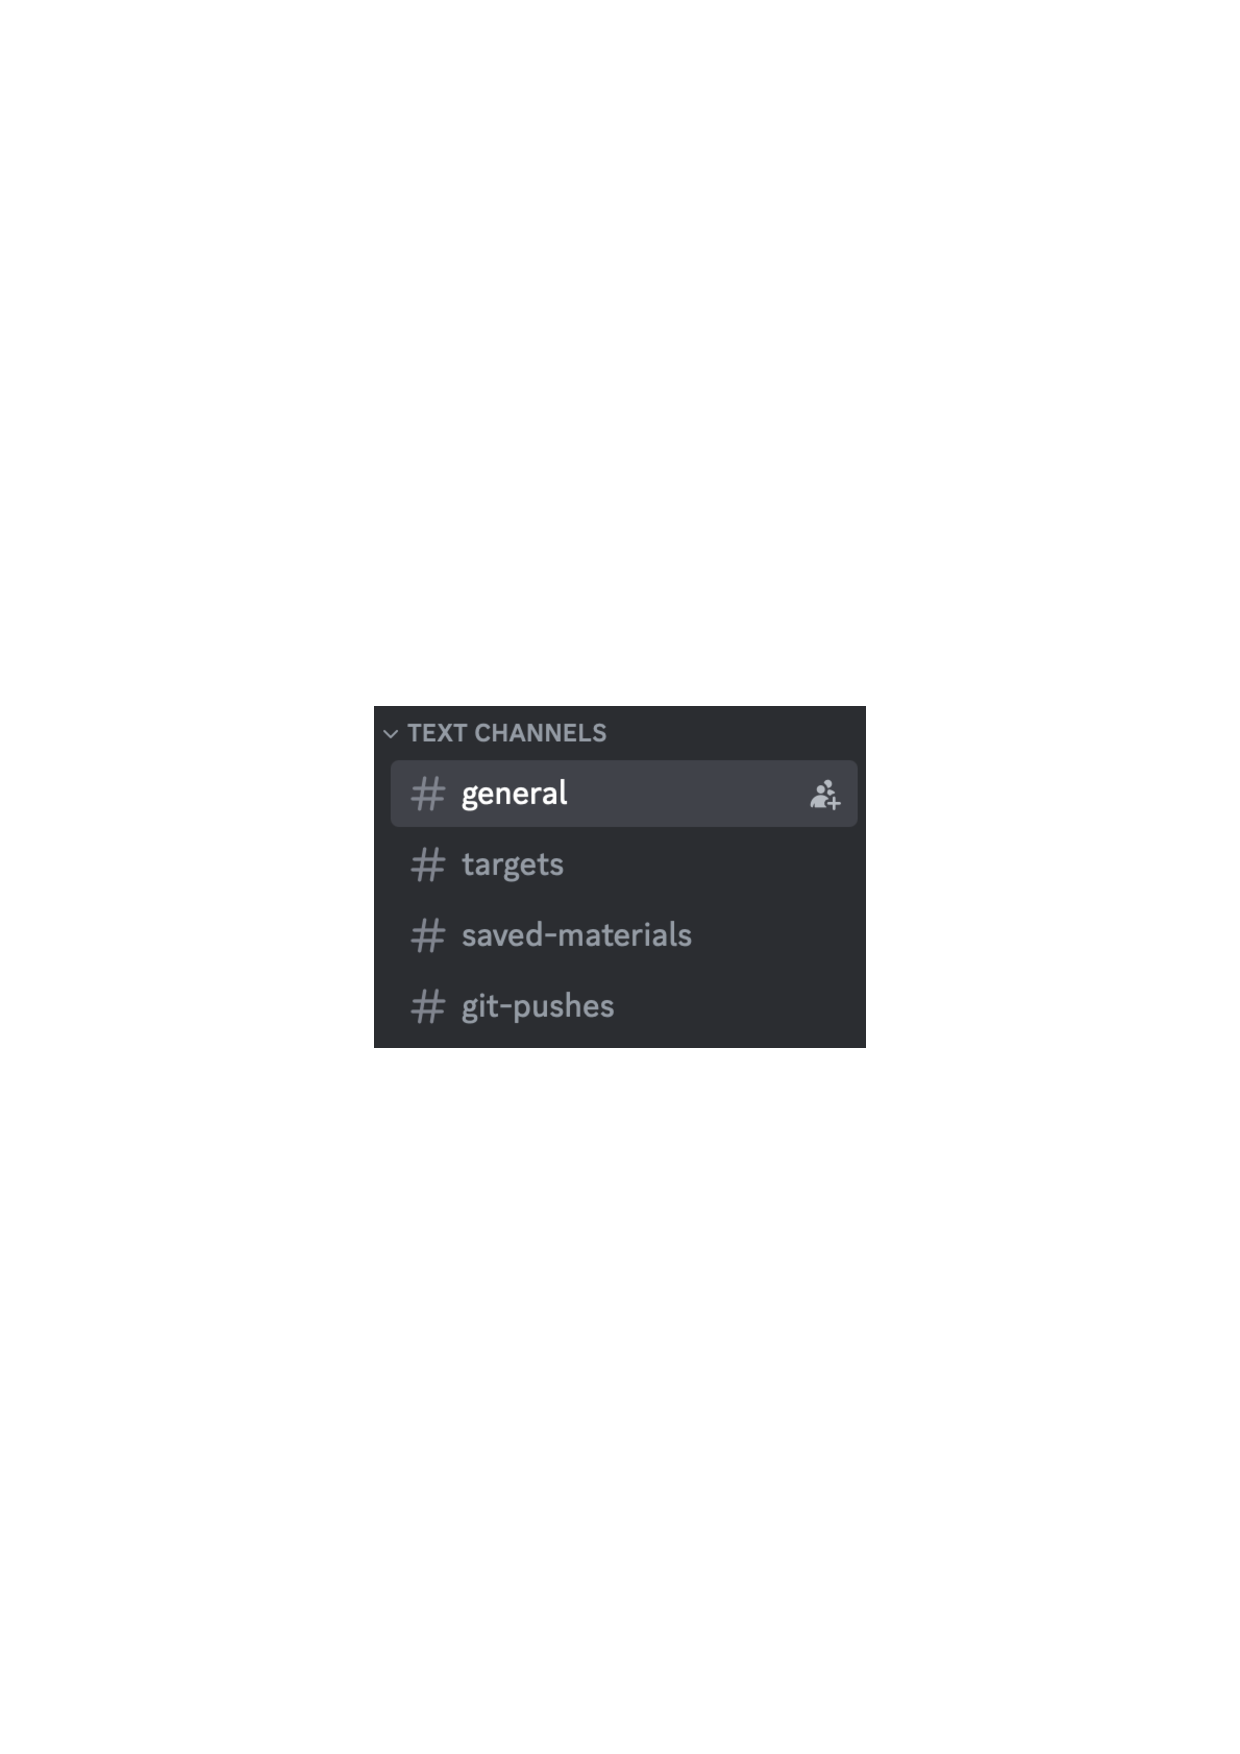
\includegraphics[width=0.7\textwidth]{resources/discord_channels.pdf}
    \caption{Different Discord communication channels used in the project}
    \label{fig:discord_channels}
\end{figure}

A critical reflection here is that, despite this plan, some members disengaged, which caused delays in certain tasks (see Section 4.2.2). This demonstrates how initial communication plans can be tested under real project conditions.

\section{Execution}
Execution involved turning our plans into tangible deliverables—writing code, creating the database structure, designing interfaces, and more.

\subsection{Task Allocation and Progress Tracking}
We adopted a weekly task allocation model at the start of each Wednesday meeting. For instance:
\begin{itemize}
    \item \textbf{Hugo:} Responsible for integrating new habit data into the MySQL database.
    \item \textbf{Doris:} Responsible for the statistics-page database functionalities.
\end{itemize}

Each person reported on progress the following week, as recorded in meeting minutes. If tasks were incomplete, we reassigned them or extended deadlines.

For evidence of this approach, see the weekly minutes excerpt below:

\begin{quote}
\textbf{Excerpt 4.1.} Individual accountability of task (Minutes 12/02/25)\\
\textit{"Action/commitment: Add selector to statistics page to pick different habits in the table.\\
Person responsible: Ming\\
Deadline: 12/02/25\\
Progress: In progress, deadline extended to 26/02/25"}
\end{quote}

This approach worked incredibly well for us, as it allowed us to keep track of individual progress, maintain accountability, and identify tasks requiring extra attention. In the future, we could enhance this method by including more detail in the ‘Progress’ section of our weekly minutes, requiring each member to specify exactly what was done. This would provide a deeper understanding of the development process.

\subsection{Dealing with Disengagement}
A challenge we faced was the partial disengagement of some team members, which manifested through missed meetings and uncompleted tasks. As recommended by agile methodologies \cite{schwaber2020scrum}:
\begin{itemize}
    \item We reassigned tasks when a member missed more than two consecutive meetings without prior notice.\\
    \textit{Example:} As recorded in Meeting Minutes 26/02/25, under New Commitments: “Reassigned calendar page task to Andrew.”
    \item We reduced the scope of certain features (e.g., scaled back the AI-based habit recommendation system).
\end{itemize}

\subsection{Ensuring Code Quality}
Initially, we planned code inspections and peer reviews for each major functionality. However, in practice:
\begin{itemize}
    \item We relied heavily on automated testing instead of thorough peer reviews.
    \item Due to time constraints, we conducted fewer formal inspections and prioritised feature completion.
\end{itemize}

In retrospect, while automated testing coverage was beneficial, face-to-face reviews could have caught inconsistencies earlier. This aligns with standard software engineering advice, which highlights that code reviews often catch design and logic flaws beyond what unit tests detect \cite{fowler2018refactoring}.

\section{Monitoring and Control}
Monitoring and control involved continuously checking our progress against the plan and adapting as needed.

\subsection{Regular Check-ins and Task Status}
Each weekly meeting served as a control point:
\begin{itemize}
    \item We reviewed completed tasks vs. planned tasks.
    \item We updated the Trello board (e.g., moving items to “Done” or reassigning them).
    \item We merged completed branches to the master branch on GitHub together, preventing serious conflicts.
\end{itemize}

\begin{figure}[H]
    \centering
    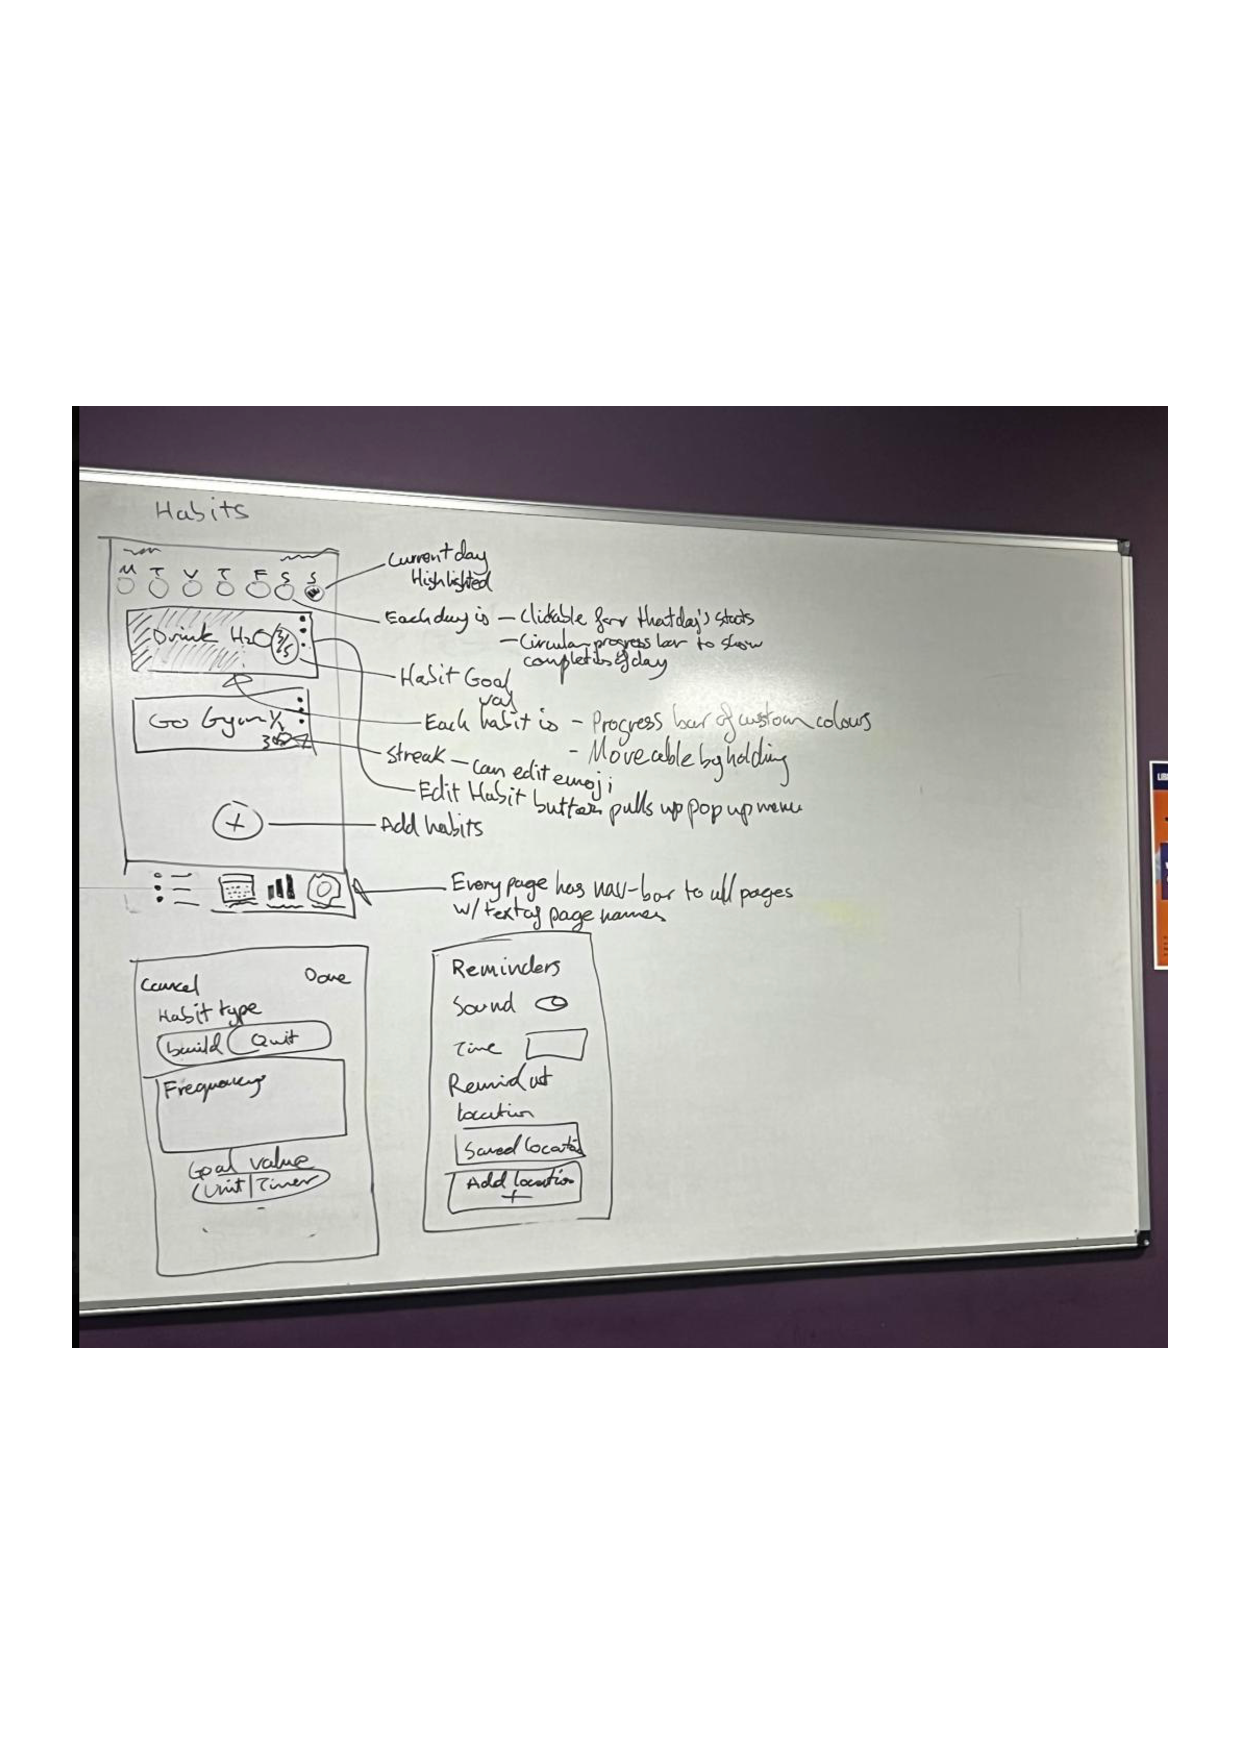
\includegraphics[width=0.7\textwidth]{resources/board.pdf}
    \caption{Designing the app during a weekly meeting}
    \label{fig:whiteboard_meeting}
\end{figure}

We conducted a project review meeting where we reassessed project risks, scheduling, and communication plans (Meeting Minutes 26/02/25). A key issue we identified was that we only held one project review meeting, which we believe was insufficient for a project of this duration. We have discovered the importance of regular reviews, as it allows us to maximise productivity by taking a look at our progress and challenges. Perhaps if more reviews were conducted, we may have caught arising issues (e.g. security risks) earlier on.

\section{Close}
Finally, closing the project required delivering the final software product and supporting materials. Whilst our official deadline is 27/03/25, we began planning for closure early to mitigate last-minute rush or errors.

\subsection{Preparing Final Deliverables}
\begin{itemize}
    \item \textbf{Codebase:} Fully merged into the main branch on GitHub.
    \item \textbf{App Deployment:} Tested on Expo Go and verified basic web accessibility.
    \item \textbf{Test Deployments:} Conducted in a staging environment.
\end{itemize}

Even though we planned for early completion, we still felt slightly rushed as a team by the end. To prevent this problem in the future, we could have set our own deadline a week prior to submission, which would allow the last week to be focused solely on refinements/polishing the deliverables.

\section{Conclusion}
Overall, our hybrid Agile/Waterfall project management strategy provided us with structure and flexibility. Despite challenges, we successfully adapted by reallocating tasks, adjusting our scope, and focusing on core deliverables. Our experience shows that a structured and thoughtful project management approach, based on best practices and real-time adaptation, is key to delivering complex software projects.






    \chapter{Design and implementation}
\label{chap:design-and-implementation}

\section{Design and Implementation}

This section discusses how our software is designed and implemented, focusing on meeting both functional requirements (such as creating and managing habits) and non-functional requirements (such as security, maintainability, and reliability). We outline the three-tier architecture and explain our rationale for each design choice, demonstrating how the client, server, and database work together.

\subsection{Overall Architecture}

Our system uses a three-tier structure: \begin{itemize} \item \textbf{Client (React Native and Expo)}:
Displays user interfaces for activities like logging in, managing habits, and viewing calendars or statistics. We use Expo Router to organise screens.
\item \textbf{Server (Node.js and Express)}:
Provides REST endpoints (for example, /signup, /addHabit, /export/:email) to handle authentication, validate user data, and manage business logic.
\item \textbf{Database (MySQL via mysql2/promise)}:
Stores user credentials, habit definitions, scheduling information, and user progress records. \end{itemize}

\begin{figure}[H]
    \centering
    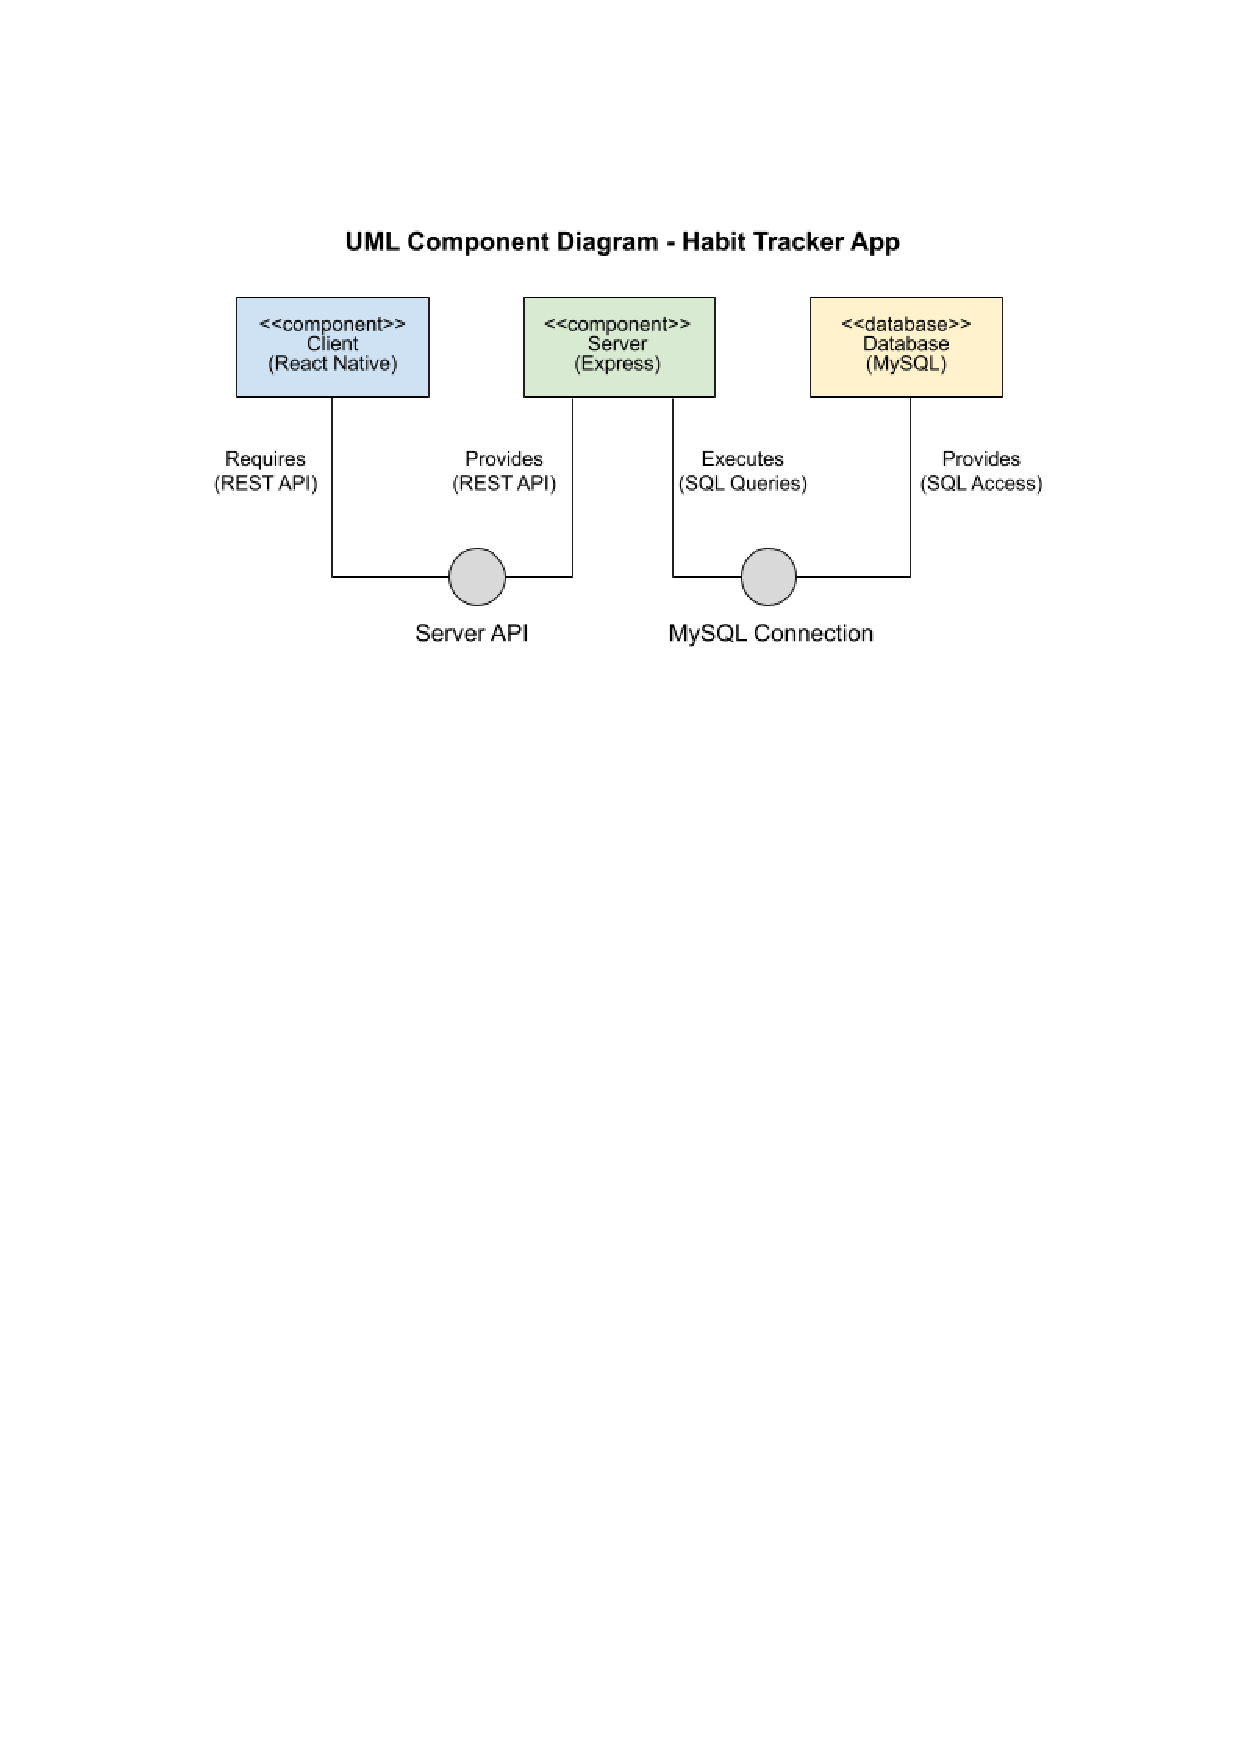
\includegraphics[width=0.7\textwidth]{resources/component.pdf}
    \caption{UML Component Diagram of our Habit-Tracker Application}
    \label{fig:component_diagram}
\end{figure}

Figure \ref{fig:component_diagram} illustrates these layers. By separating the UI (client), the application logic (server), and storage (database), each layer remains independently maintainable and secure.

\subsection{Key Design Decisions}

\subsubsection{Cross-Platform Client Using Expo:}

\paragraph{Choice and Reasoning} \begin{itemize} \item We wanted a single codebase (TypeScript) for iOS, Android, and web accessibility, which is why we chose React Native and Expo.
\item Expo simplifies building and testing on multiple platforms, preventing the need for a complicated setup. This allowed us to start developing features much sooner, rather than spending time on configuration.  \end{itemize}

\paragraph{Implementation Details} \begin{itemize} \item {File Structure}:
\begin{itemize} \item {src/app/(auth)/}: Handles login and signup screens.
\item{src/app/(protected)/tabs/}: Contains the main habits, calendar, stats, and settings screens.
\item{src/components/}: Contains reusable UI elements such as habit modals, calendars, graphs, themed text, and shared styles for consistent design.
\item {src/lib/client.ts}: Centralises HTTP request logic to avoid repeating fetch calls across components. \end{itemize} 
This modular structure improves code organisation, makes features easier to maintain, and encourages reuse of components across the app, as shown in the SOLID design principles \cite{martin2002solid}.

\item {Styling and Theming}:
\begin{itemize} 
\item The app uses shared colours and styles so that all screens look consistent.
\item Common layouts, buttons, and inputs are defined in reusable style files to avoid repeating code.
\item Some components automatically change their appearance based on the selected theme (light or dark), making the app easier to use and nicer to look at. \end{itemize} \end{itemize}


\subsubsection{Server with Node.js and Express:}

\paragraph{Choice and Reasoning}
\begin{itemize}
\item Node.js and Express were chosen because they are widely used, beginner-friendly, and well-supported by online documentation and learning resources.
\item Express enables a simple and flexible REST API structure, making it easy to define endpoints that connect to application features like signing up, adding habits, or exporting data.
\end{itemize}

\paragraph{Implementation Details}
\begin{itemize}
\item Express is used to define REST endpoints such as \texttt{/signup}, \texttt{/addHabit}, and \texttt{/export/:email}, which the client interacts with to manage user accounts and habits.
\item Middleware like \texttt{cors} and \texttt{dotenv} help with handling requests, loading environment settings, and allowing the mobile app to connect to the server.
\item Authentication uses JSON Web Tokens (JWT) to protect routes and make sure only logged-in users can access certain features.
\end{itemize}

\subsubsection{MySQL Database:}

\paragraph{Choice and Reasoning}
\begin{itemize}
  \item A relational database structure is ideal for managing related entities such as users, habits, and habit completion logs. MySQL allows us to enforce clear relationships and constraints through primary and foreign keys.
  
  For example, in the habit\_progress table, a foreign key constraint on (user\_email, habitName) references the habits table. This ensures that progress entries cannot exist without a matching habit, and enables automatic cleanup of related records when a habit is deleted, maintaining data integrity.

  \item We use the \texttt{mysql2/promise} library to write our own SQL commands directly (such as \texttt{CREATE TABLE} and \texttt{SELECT}) and run them using modern \texttt{async/await} syntax. This gives us full control over database operations, and keeps the code clean, readable, and easier to debug.
\end{itemize}

\paragraph{Schema Outline}\mbox{}\\
Below is an overview of some of the main tables that make up our database schema.
\begin{itemize}

  \item {users}: Stores user account information. The \texttt{email} field acts as the primary key and is used to identify users. Each user also has a hashed password and a username.

  \item {habits}: Stores details about each habit a user creates. Each habit is uniquely identified by a combination of \texttt{user\_email} and \texttt{habitName}, which together form a composite primary key. Other fields include habit type (build or quit), goal settings, and scheduling options (e.g., interval or weekly).

  \item {habit\_progress}: Logs daily progress for each habit. The composite primary key (\texttt{user\_email}, \texttt{habitName}, \texttt{progressDate}) ensures that only one record exists per user, habit, and date. This table tracks goal progress, completion status, and streak count. A foreign key links back to the \texttt{habits} table, ensuring referential integrity.

\item {habit\_days}: Supports weekly habit scheduling. Each record maps a habit to a day of the week (e.g., Monday, Wednesday). This allows habits to repeat on specific days, and also uses a foreign key to maintain referential integrity with the \texttt{habits} table.

\end{itemize}

\begin{figure}[H]
    \centering
    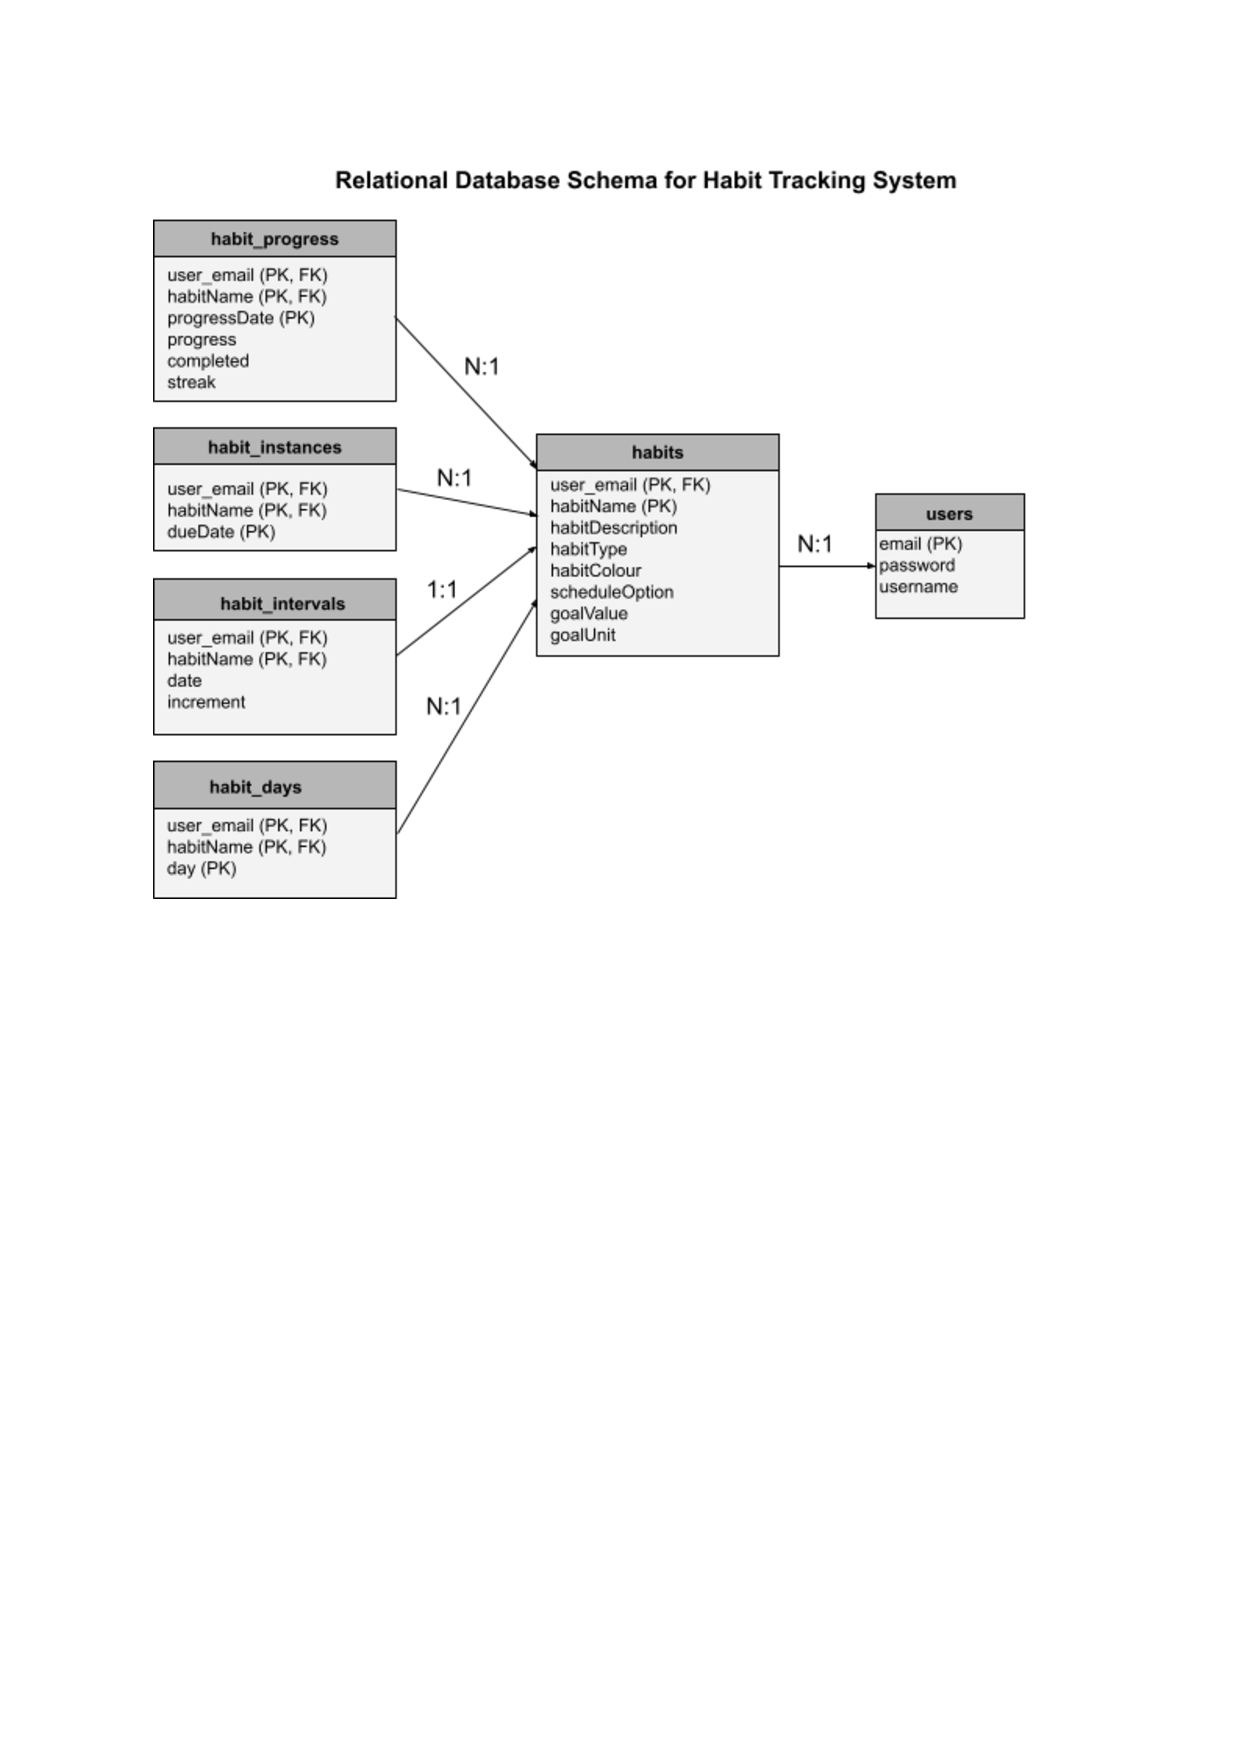
\includegraphics[width=0.9\textwidth]{resources/database_schema.pdf}
    \caption{Relational Database Schema of our Habit Tracking System}
    \label{fig:database_schema}
\end{figure}

Figure \ref{fig:database_schema} shows the tables in the habit-tracking database and their relationships. Arrows represent foreign keys, and cardinality ratios (e.g., 1:1, N:1) indicate how records in one table relate to others, supporting data integrity and structure.

\section{Meeting Requirements}

This section summarises some examples of how our system design and implementation meet the project's key functional and non-functional requirements (as specified in Chapter 3 of this report). We focus on how our architecture, database structure, and code design support these goals (instead of just listing all the features).

\subsection{Functional Requirements}

\begin{itemize}
  \item \textbf{Habit Creation and Management:} Users can create, customise, and update habits with flexible scheduling (interval-based or weekly), goals, and visual settings. These features are implemented through reusable client components and backed by structured database tables (\texttt{habits}, \texttt{habit\_progress}, \texttt{habit\_days}).

  \item \textbf{Progress Tracking and Visualisation:} The system calculates and displays daily progress, streaks, and completion trends via calendar views and graphs. These visual features reflect real-time data stored and retrieved from the backend.

  \item \textbf{Data Export:} A dedicated API endpoint (\texttt{/export/:email}) allows users to download their habit history in JSON format, so users can view and save a copy of their own data.
\end{itemize}

\subsection{Non-Functional Requirements}


\begin{itemize}
  \item \textbf{Security:} All user passwords are hashed client-side before being sent to the server. Routes requiring authentication use JSON Web Tokens (JWT), and all data operations go through validated REST endpoints.

  \item \textbf{Maintainability:} The codebase is modular, with clear separation between client, server, and database logic. Client-side fetch logic is centralised, and components follow single-responsibility principles for easier reuse and testing.

  \item \textbf{Performance and Scalability:} We use SQL with \texttt{mysql2/promise} to make database queries fast and efficient. Composite keys and foreign key links help keep the data consistent and quick to access.

  \item \textbf{Data Integrity:} Relationships between tables are enforced through composite foreign keys. For example, \texttt{habit\_progress} entries reference existing habits, and \texttt{ON DELETE CASCADE} ensures cleanup when habits are removed.
\end{itemize}


\section{Alternative Approaches}

Throughout development, we considered several alternative technologies and approaches:

\begin{itemize}
  \item {Using an ORM}: ORMs can make database tasks easier, but we chose to write SQL ourselves using \texttt{mysql2/promise} to have more control over scheduling logic and table relationships like composite keys and foreign keys.

  \item {Native iOS/Android Development}: We considered building separate native apps for each platform, but chose React Native with Expo to keep one shared codebase. This made development easier and faster, while also allowing the app to run smoothly on iOS, Android, and the web.
\end{itemize}


\section{Conclusion}

Our design and implementation emphasise a three-tier architecture that separates the user interface, server-side logic, and database.
The result is a cross-platform habit-tracking application that cleanly meets project needs for scheduling, progress tracking, data visualisation, and security measures. The system is also designed to be easily extended in the future, with potential additions like advanced analytics, social features, or smarter notifications.

    \chapter{Testing}
\label{chap:testing}

This chapter describes the testing approaches we used to ensure our habit-tracking application is reliable and working as expected. Throughout our development, we combined automated testing (using Jest, React Native Testing Library, and mocks) with targeted manual tests for cross-platform validation. While our automated coverage is high, our critical reflection reveals areas where we could have improved our quality assurance process.

\section{Approach and tools} \label{sect:testing:approach}

\subsection{Automated Testing}

We relied heavily on automated testing to make sure our features worked as expected. Each suite checks how the component renders, responds to user actions (e.g., button presses), and triggers any side effects (like functions in \texttt{lib/client}). This approach helps us confirm that our UI logic, data calls, and component behaviours work as intended.

\paragraph{Tools Used} \begin{itemize} \item \textbf{Jest}: Our main test runner, responsible for executing the test suites. \item \textbf{React Native Testing Library}: Lets us simulate user interactions (like tapping buttons or typing text). \item \textbf{Some examples of our Mocking Techniques}: \begin{itemize} \item{AsyncStorage}: Replaces native storage calls so tests don’t fail on missing native modules. \item{Fetch}: Fakes server API calls, which means our tests do not depend on a real network. \item {Expo Router and ThemeContext:}
We replace real navigation and theming with simple "fake" versions. This way, our tests focus only on the component’s behavior, rather than on actual screen transitions or styles. \item {Victory Charts}: This library uses SVG (Scalable Vector Graphics) to draw charts. In our tests, we swap the real chart components for simpler “mocks.” This means the charts don’t actually get rendered, and our tests run faster with fewer errors. For example, in \texttt{BuildHabitGraph.test.tsx}, we check that the chart component receives the right data without drawing any real SVG. \end{itemize} \end{itemize}


\paragraph{Location of Automated Tests}\mbox{}\\

We keep our tests in the \texttt{client/src/components/\_\_tests\_\_} folder, and we name each file after the component it tests. For example:

\begin{itemize} \item \texttt{BuildHabitGraph.test.tsx}\item \texttt{WeeklyCalendar.test.tsx} \item \texttt{SettingsPage.test.tsx} \end{itemize}

This structure makes it easy to locate each test and ensures that test code remains closely tied to its corresponding component.

One critical reflection is that we did not integrate automated testing as thoroughly as we had hoped during development. Although we did test throughout the entire project, many tests were only added later in the project, which in hindsight left some functionalities untested for longer than we would have liked.

\subsection{Manual Testing}

While automated tests validate most of our components and logic, we supplemented them with manual testing to ensure the application feels correct when being used. Each major functionality (e.g., habit creation, editing, exporting data) was checked on iOS, Android, and the web).

\paragraph{Limits of Manual Testing}\mbox{}\\
Although manual checks can uncover issues that automated tests might miss, such as subtle design issues or platform-specific bugs, this approach is slow and difficult to maintain for every new change, as Crispin and Gregory point out \cite{crispin2009agiletesting}. As a result, we focused our manual testing on critical features and cross-platform validation, rather than using it for every update.

\subsection{Test Coverage Report} \label{sect:test-coverage} 
\begin{figure}[H]
    \centering
    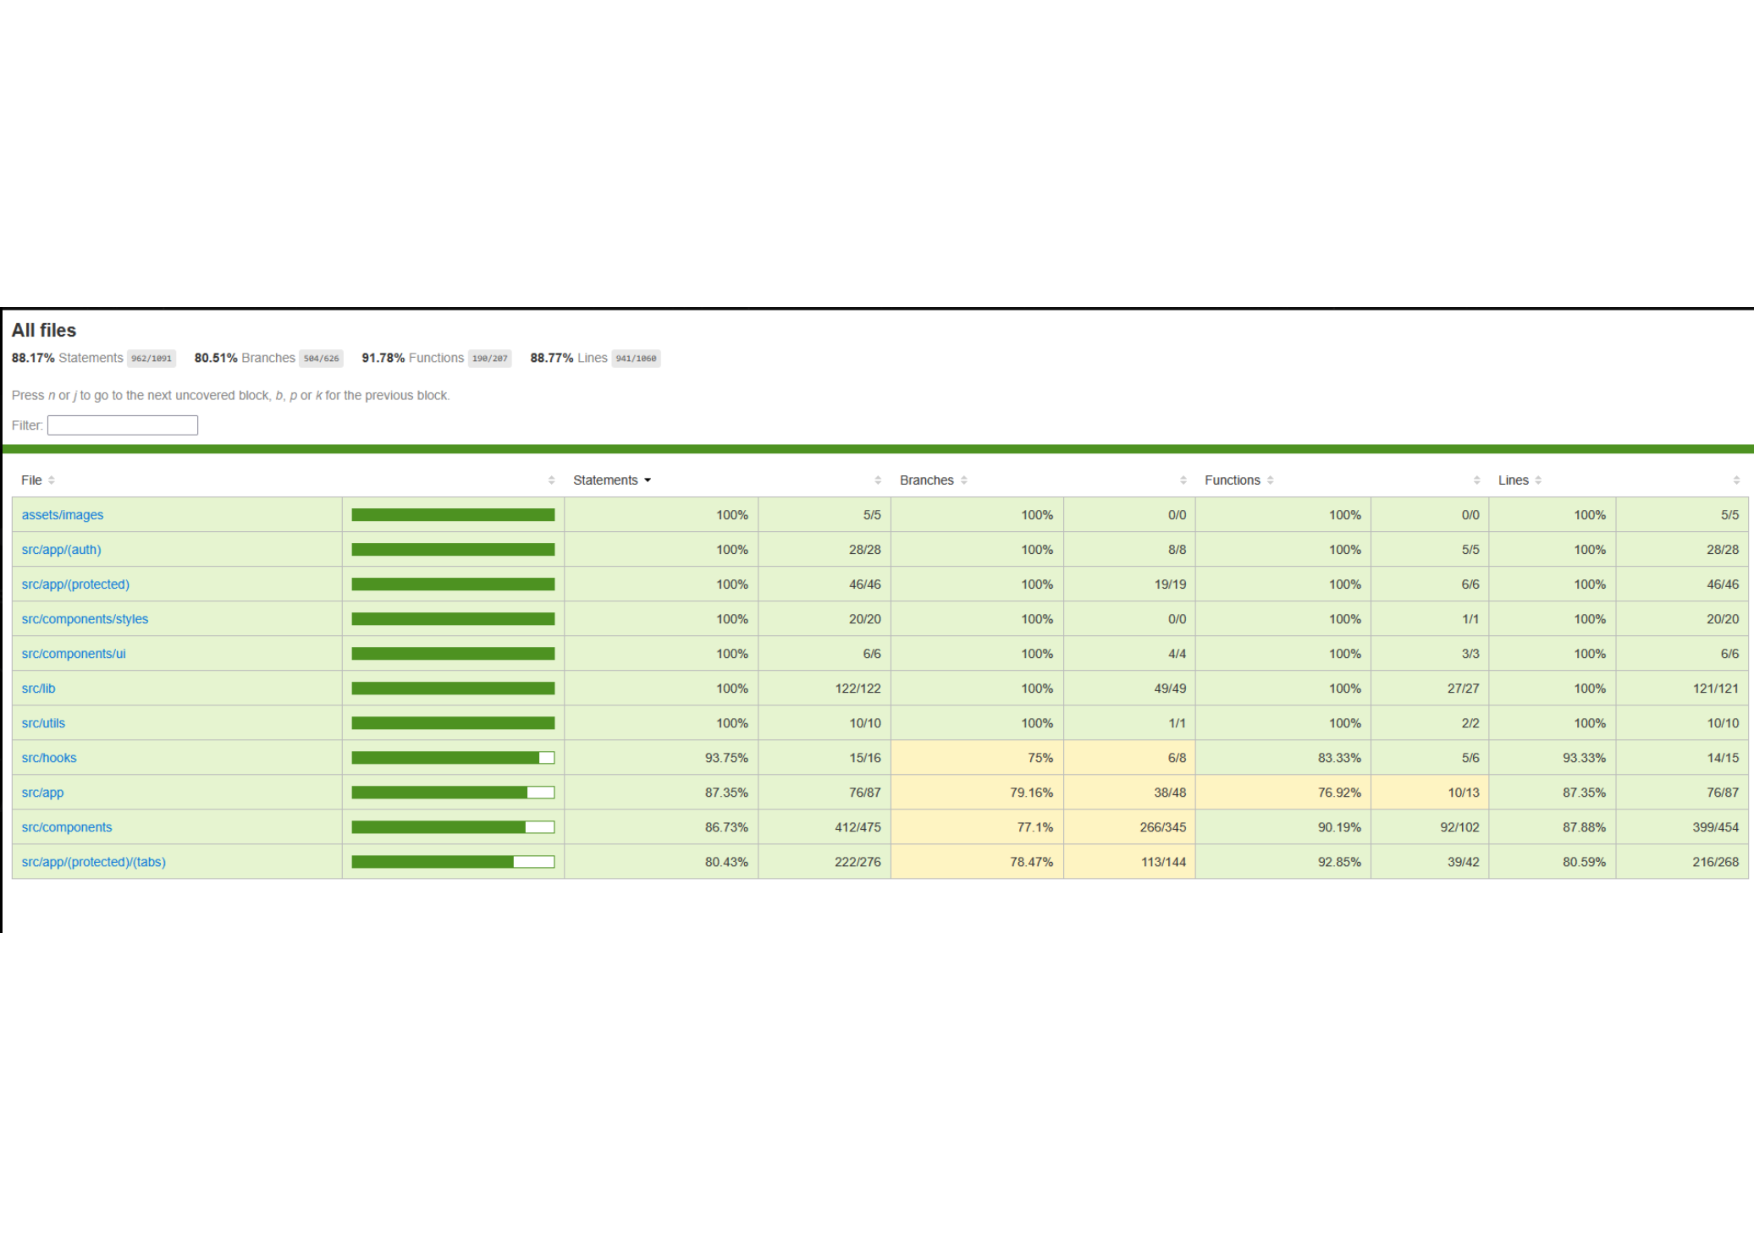
\includegraphics[width=0.7\textwidth]{resources/test_coverage.pdf}
    \caption{Test Coverage Report of our Habit-Tracker Application}
    \label{fig:test_coverage}
\end{figure}

Figure \ref{fig:test_coverage} shows our test coverage report. The source coverage details (HTML pages) are located in the project’s coverage/lcov-report folder, particularly in the index.html file. 


\section{Evaluation of testing} \label{sect:testing:evaluation}

\subsection{Strengths} \begin{itemize} \item \textbf{Extensive Automated Coverage}: Our Jest tests are well-integrated, ensuring we can trust most core functionalities. Mocking external dependencies (network, storage, theming) keeps our tests deterministic and easier to maintain. \item \textbf{UI Testing}: By using React Native Testing Library, we test not just logic but actual user interactions (tapping buttons, text input, etc.). \item \textbf{Cross-Platform Verification}: Manual checks on iOS, Android, and web prevent platform-specific issues and ensures a consistent experience. \end{itemize}

\subsection{Weaknesses and Reflections} \begin{itemize} \item \textbf{Fewer Formal Inspections}: We relied heavily on automation due to limited time. This left less room for structured peer review or code inspection, which can catch architecture-level or readability issues that tests miss. \item \textbf{Lack of External Black-Box Testing}: Although we occasionally showed demos to family/friends, we did not organise a broader group of external testers. This might have revealed usability issues or inconsistencies that a developer-focused approach could overlook.\end{itemize}

\subsection{Future Improvements} \begin{itemize} \item \textbf{More Peer Reviews}: In future we would review each other’s pull requests more often and thoroughly, which could reduce hidden defects early on. \item \textbf{Black-Box Testing:} Bringing in more people who haven’t seen our code would provide fresh perspectives and more thorough user feedback. \item \textbf{Formalising Manual Test Cases}: Storing each manual test case (actions, expected results) in a shared document would add clarity and accountability for each test run.
\item \textbf{Automated Testing during Development}: We would prioritise the need test more thoroughly throughout the entire project, making sure no functionalities were left untested for longer than necessary.\end{itemize}

\noindent Overall, our mix of automated tests and manual checks gave us confidence in our software’s correctness and stability. However, we recognise that further improvements could be made to our testing to strengthen our quality assurance.
    % \chapter{Machine learning}
\label{chap:machine-learning}

\defaultInstructions

\begin{instructions}
By default, this chapter is not included in the report because most teams do \emph{not} need this chapter.  If your project requires this chapter, uncomment the \texttt{input} command that includes this chapter.
\end{instructions}

\begin{expectations}
If your project includes training a machine learning model, and you made an effort to evaluate alternative  approaches, teams should include this chapter discussing the machine learning work.  It is recommended to  include a short summary description for each considered approach, a clear description and rationale of the  approach taken to evaluate and compare the different algorithms, a table summarising the results obtained in evaluation, and your team's decision on what algorithm was chosen for incorporation in the system.  Also  explain how the team's results can be replicated.  This chapter is not required if an existing machine learning model or tool was used, or if the team did not evaluate the machine learning component.
\end{expectations}  % Uncomment this line if you need this chapter.

    \appendix
    % \chapter{Manual tests}
\label{chap:manual-tests}

\defaultInstructions

\begin{instructions}
By default, this chapter is not included in the report because many teams do \emph{not} need this chapter.  If your project requires this chapter, uncomment the \texttt{input} command that includes this chapter.
\end{instructions}

\begin{expectations}
If your team relied on manual testing, and the manual testing was carefully planned such that the team has a detailed written specification of its tests, then this chapter should be used to provide a list of all the team's tests.  A template table is provided to help format the tests.
\end{expectations}

\begin{longtable}{| p{.04\textwidth} | p{.40\textwidth} | p{.25\textwidth} | p{.18\textwidth} |} 
\hline
\# & Test script & Expected outcome & Outcome/date \\ \hline
\endhead
1 & Specify the actions the tester must undertake to run the test. & Specify what the tester must observe. &  \\ \hline
\end{longtable}  % Uncomment this line if you need this chapter.
\end{document}
